\chapter{Introduction}
\label{chap:introduction}

\section{Background}
Osteoarthritis is commonly recognised after symptoms or structural changes
become established. A hypothetical research programme might test whether
quantitative magnetic resonance imaging can identify earlier tissue changes.
The condition affects the whole joint rather than cartilage alone, so a useful
study would combine structural, compositional, mechanical and patient-reported
measures.

This sentence demonstrates a footnote.\footnote{Footnotes appear at the bottom
of the page in smaller, single-spaced text. They are numbered automatically and
should contain information needed to understand the corresponding passage.}

\ifbrightonbiblatex
  The example journal article is cited narratively using
  \textcite{example2026}. A book and an online source demonstrate citations in
  parentheses \parencite{examplebook2025;exampleweb2026}. A direct quotation
  should include a page number \parencite[p.~6]{example2026}.
\else
  The example bibliography is demonstrated using Example Author (2026).
\fi

Figure~\ref{fig:pathway} demonstrates automatic figure numbering. Its caption
also creates an entry in the list of figures.

\begin{figure}[htbp]
  \centering
  \setlength{\unitlength}{1mm}
  \begin{picture}(118,34)
    \put(0,8){\framebox(30,16){Risk factors}}
    \put(30,16){\vector(1,0){14}}
    \put(44,8){\framebox(30,16){Early change}}
    \put(74,16){\vector(1,0){14}}
    \put(88,8){\framebox(30,16){Symptoms}}
  \end{picture}
  \caption{Illustrative pathway from risk factors to symptomatic disease}
  \label{fig:pathway}
\end{figure}

\section{Rationale}
\label{sec:rationale}
Early identification is valuable only if an imaging signal can be reproduced,
interpreted clinically and associated with a meaningful later outcome.
Consequently, an example thesis might distinguish three linked questions:

\begin{enumerate}
  \item Can early tissue change be measured reliably?
  \item Does that measure predict symptoms or structural progression?
  \item Does it add information beyond routine clinical assessment?
\end{enumerate}

\subsection{Clinical context}
\label{sec:clinical-context}
Osteoarthritis illustrates why a single observation rarely provides a complete
account of disease. Symptoms, structural findings and function may change at
different rates. A clinically useful study must therefore explain who is being
assessed, when assessment occurs and how an imaging result might alter a
decision. The following demonstrates an unordered list:

\begin{itemize}
  \item symptoms reported by the participant;
  \item structural features visible on conventional imaging;
  \item compositional features measured using quantitative MRI; and
  \item contextual factors such as age, previous injury and mechanical load.
\end{itemize}

\subsubsection{Symptoms and function}
Pain intensity, stiffness and activity limitation describe related but distinct
parts of the participant's experience. A thesis should define each outcome,
identify the instrument used and state the time point to which it relates.

\subsubsection{Structural assessment}
Radiographs and morphological MRI sequences can describe established structural
features. Their interpretation should include information about acquisition,
reader training and repeatability.

\subsubsection{Compositional assessment}
Quantitative sequences may be sensitive to tissue changes that precede gross
structural loss. Their value depends on measurement reliability and evidence
that the signal predicts an outcome important to patients. This is the third
subsubsection under Section~\ref{sec:clinical-context}, so its automatically
generated number ends in ``.3''.

\subsection{Conceptual framework}
A conceptual framework makes assumptions visible before analysis. In this
example, exposure and susceptibility factors may influence early tissue change,
which may in turn affect later symptoms and function. Potential confounders
should be identified from subject knowledge rather than selected solely from
observed statistical associations.

\subsection{Translation to study design}
The framework can then be translated into a sampling strategy, measurement
schedule and analysis plan. This subsection is deliberately included as the
third subsection of Section~\ref{sec:rationale}, demonstrating an automatically
generated heading numbered 1.2.3.

Figure~\ref{fig:joint-model} demonstrates a more detailed diagram created
directly in LaTeX using TikZ. Because it is vector artwork, it remains sharp at
any zoom level.

\begin{figure}[htbp]
  \centering
  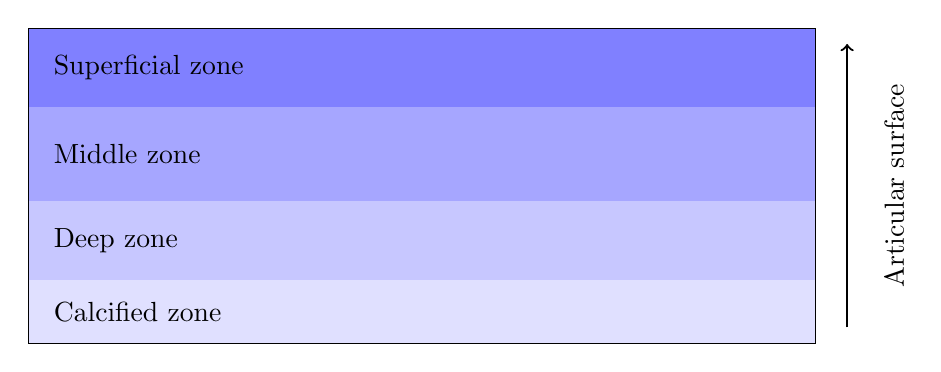
\begin{tikzpicture}[x=1cm,y=1cm]
    \fill[blue!12] (0,0) rectangle (10,0.8);
    \fill[blue!22] (0,0.8) rectangle (10,1.8);
    \fill[blue!35] (0,1.8) rectangle (10,3.0);
    \fill[blue!50] (0,3.0) rectangle (10,4.0);
    \draw (0,0) rectangle (10,4);
    \node[anchor=west] at (0.2,0.4) {Calcified zone};
    \node[anchor=west] at (0.2,1.3) {Deep zone};
    \node[anchor=west] at (0.2,2.4) {Middle zone};
    \node[anchor=west] at (0.2,3.5) {Superficial zone};
    \draw[->,thick] (10.4,0.2) -- (10.4,3.8);
    \node[rotate=90] at (11.0,2.0) {Articular surface};
  \end{tikzpicture}
  \caption{Schematic representation of the zones of articular cartilage}
  \label{fig:joint-model}
\end{figure}

\section{Research question}
State the primary research question and objectives. A simple mathematical
example is
\begin{equation}
  R = \alpha I + \beta M + \gamma S.
  \label{eq:risk}
\end{equation}

\begin{brightonquotation}
Indented quotations and footnotes may use single spacing under the Brighton
requirements.
\end{brightonquotation}

Equation~\ref{eq:risk} is numbered automatically and can be cited from any
chapter.

\subsection{Example objectives}
The description-list format is useful when each item needs a short label
followed by an explanation:

\begin{description}
  \item[Objective 1] Estimate the repeatability of the quantitative imaging
    measure under a prespecified acquisition protocol.
  \item[Objective 2] Test its association with change in symptoms and structure
    over 24 months.
  \item[Objective 3] Assess whether it adds useful predictive information to
    routinely available clinical variables.
\end{description}

\section{Chapter summary}
The chapter has demonstrated several paragraphs of ordinary prose, three levels
of numbered heading, ordered, unordered and description lists, two types of
figure, a quotation, a footnote, an equation and cross-references. The source
file remains independent from the other chapters while all numbering is
controlled by \texttt{main.tex}.
